\documentclass[11pt]{article}
\usepackage{memo}

% Parmaters --
\title{\large\textbf{Survey Weighting for (Moderately Large) Subnational Samples}}
\author{\normalsize  Shiro Kuriwaki\thanks{Ph.D. Candidate, Department of Government and Institute of Quantitative Social Science, Harvard University. Thanks to Soichiro Yamauchi for helpful discussions.}}
\date{\normalsize December 2019}

\begin{document}

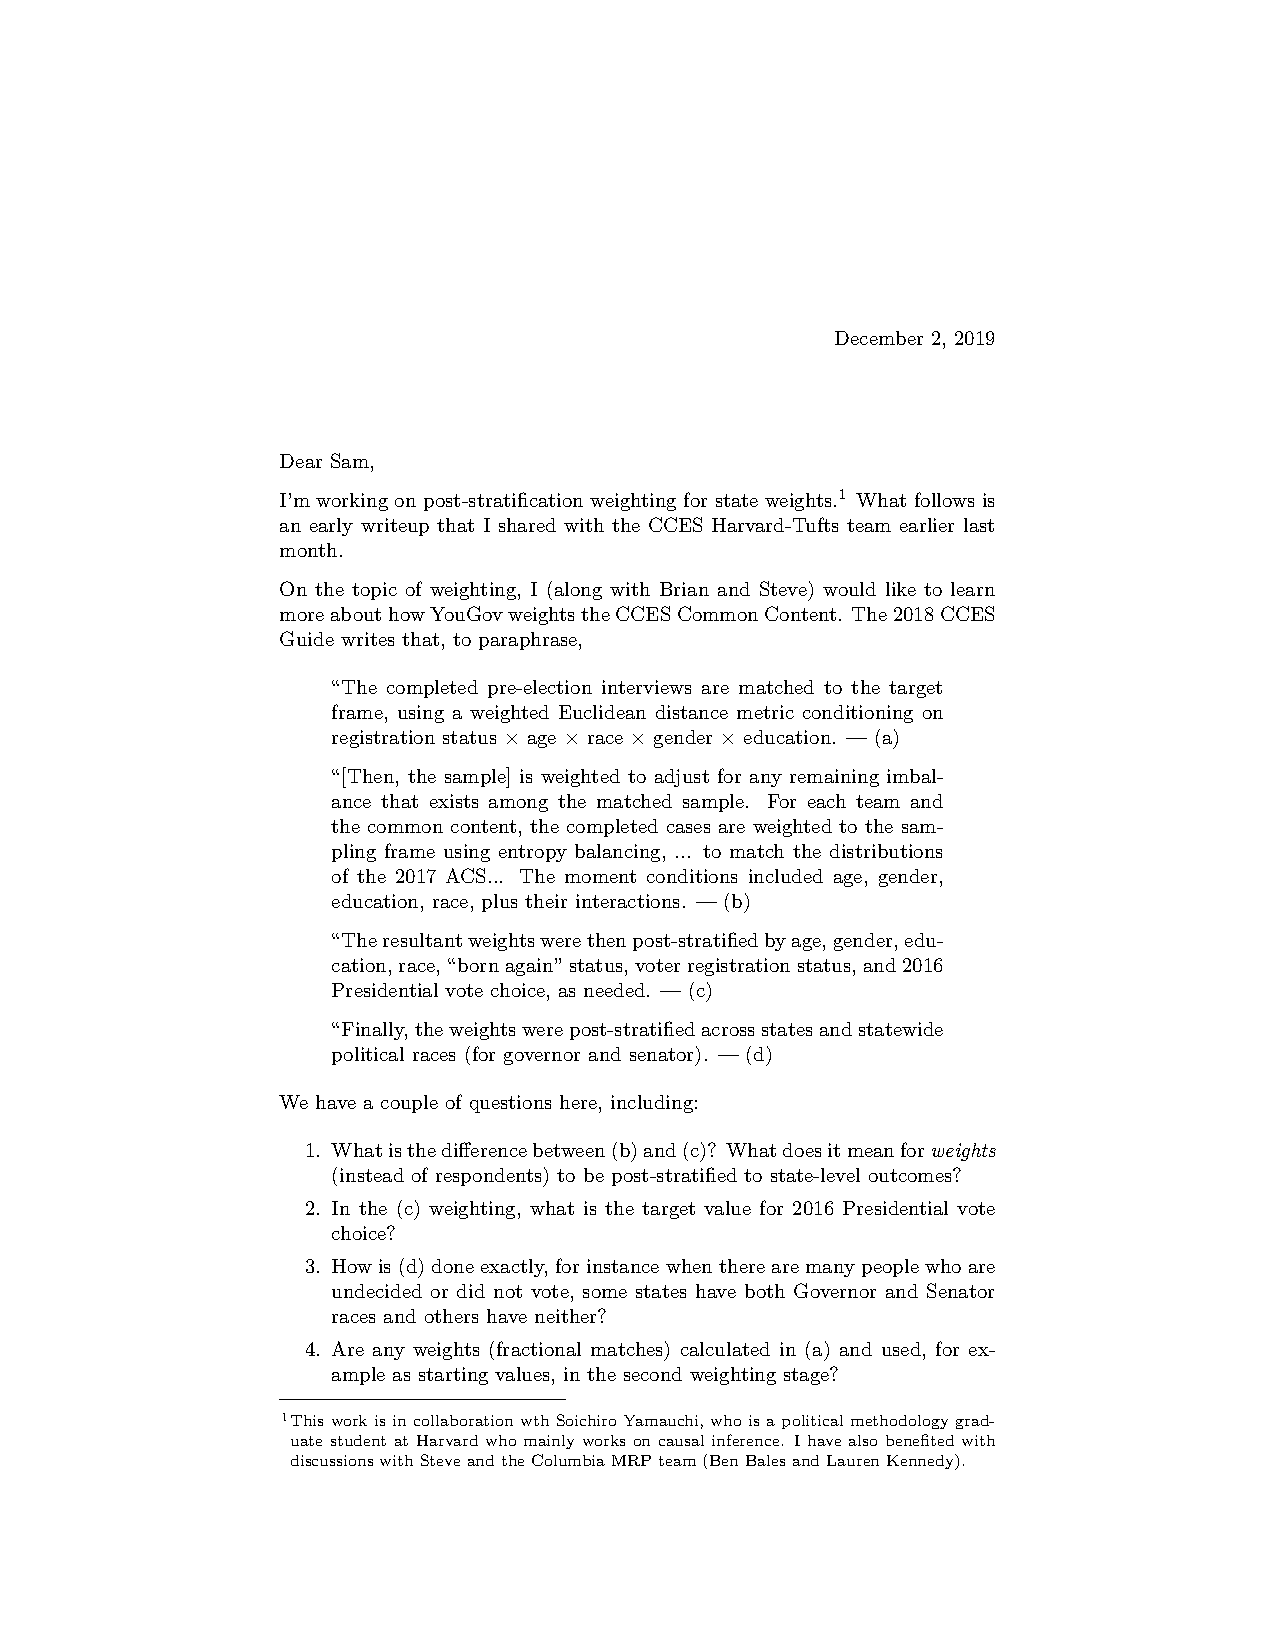
\includepdf[pages = {1, 2}]{2019-12-01_yougov-letter.pdf}


\newpage

\maketitle

\begin{abstract}
\noindent Although researchers routinely used post-stratification weights provided by survey firms, these only weight to the national adult population. When researchers attempt to estimate quantities at the subnational level, they either (a) erroneously apply national weights to subnational subsets of the survey or (b) conduct multi-level regression post-stratification (MRP). Here, using YouGov's weights for the CCES and creating my own state-level weights, I demonstrate how doing the former may skew samples less representative than no weights at all, and I clarify how doing the former latter can replaced by estimating a new set of weights directly targeted towards each geographies. MRP and post-stratification weights have opposite consequences:  MRP trades off unbiasedness for lower variance, while weighting trades off efficiency for less bias.  While post-stratification weights cannot be used for small groups, they are useful for somewhat larger geographies such as state. 
\end{abstract}

\newpage

\onehalfspacing

In this memo I explore how representative CCES samples are at subnational geographies, and whether post-stratification weights ameliorate the problem. Although post-stratification weights are designed to coerce samples to be representative, one set of weights makes a sample representative to only one target, in CCES' case the entire U.S. It is not clear if those same weights \emph{also} make subgroup samples representative of their respective subgroup targets. 

It is hard to discuss or propose survey weighting without comparing it to the increasingly popular method of Multi-level Regression Post-stratification (MRP).  In many cases, MRP is preferable to weighting because of its flexibility in combining granular post-stratification cells. However, MRP has several limitations relative to a weighting approach. First, often times analysts only have marginal, not joint, distributions as targets, namely partisanship and turnout. Second, one MRP model is specific to one outcome, so projects that involve multiple outcome questions would involve building as many multi-level models as there are outcomes. In contrast, once post-stratification weights are defined, it can be used for any sets of outcomes. 

The rest of this memo has several (currently not very well conneected) parts. In Section \ref{sec:mrp-weighting}, I compare MRP and weighting. In Section \ref{sec:methods}, I review how YouGov creates its weights and how I construct state rim weights to mirror that process. In Section \ref{sec:res-yougov}, I evaluate how YouGov weighting affects the representativeness of different subnational geographies. In Section \ref{sec:res-state}, I do the same evaluation but for rim weights. 


\section{Post-stratification Weights and MRP \label{sec:mrp-weighting}}

Each method has its pros and cons, summarized by the following table:

\begin{table}[!h]
\centering
\small
\begin{tabularx}{0.97\linewidth}{p{7cm}lCC}
\toprule
&~& (Unpooled) Weighting & MRP \\\midrule
Applying to different outcomes & & Easy, one-stop & Hard, per outcome\\
Applying to different subgroups & & Hard, per geography & Easy, one-stop\\
Pools respondents from different geographies? & & No & Yes\\
Impose modeling assumptions on... & & The selection model & The outcome model \\
Bias-variance tradeoff & & {Low bias for more variance} & {Lower variance for more bias}\\
\bottomrule
\end{tabularx}
\end{table}

The first two rows are about practicality. Weights are easy to apply to different outcomes (i.e. questions) because once constructed, researchers can apply it to all questions. In contrast, for MRP requires one model per outcome. For example, there needs to be one multilevel regression model for voting for Presidential vote choice, another for Governor vote choice, and so on. In contrast, weights are tedious to apply for different subgroups. Although it is not well-understood in practice, a single vector of weights cannot simultaneously weight to different targets. For example, if we were to explicit weight the entire CCES to each state-specific distribution, we would need 50 columns of weights, one for each state. In contrast, once an MRP model is constructed for a given outcome, it can be flexibly applied to any geography or subgroup in the geography because it makes predictions for each cell. 

The third to fifth in the table addresses the assumptions being made and their consequences. In typical weighting, there is a weight attached to each observation and observations are not pooled (i.e. a respondent in Iowa is not used as a component to estimate outcomes in Wisconsin). This lowers bias because it does not risk carrying unobserved confounding into the estimate, but increases variance. MRP pools respondents, which improves precision (which is a severe problem in small geography) at the cost of making an ignorability-on-observables assumption and risking some unobservable bias due to pooling.


\section{Setup and Methodology \label{sec:methods}}

The goal of the rest of this memo is to document how weighting affects the distribution of covariates at different sub-geographies. I do not discuss MRP here --- this is because the joint distributions of the covariates that are available are matched exactly by construction, and the worry for MRP is about the outcome model, not the weighting model.

% The ACS and CCES collect the following shared variables about their respondents. There is some difference in question wording or lumping categories, but here for simplicity I use the most common denominator.

\begin{comment}
\setlist{nosep, leftmargin = 0.5cm}

\begin{table}[!h]
\small
\begin{tabularx}{\linewidth}{XXX}
Gender & Age & Education\\\midrule
\begin{itemize}
\item Male
\item Female
\end{itemize} &
\begin{itemize}
\item 18 to 24 years
\item 25 to 34 years
\item 35 to 44 years
\item 45 to 64 years
\item 65 years and over
\end{itemize} &
\begin{itemize}
\item No high school
\item High school graduate
\item Some college, no degree
\item Associate's degree
\item Bachelor's degree
\item Graduate / professional
\end{itemize}
\end{tabularx}
\end{table}
\end{comment}


\noindent In this memo, I  consider three types of estimates:

\begin{enumerate}
\item Unweighted sample proportions
\item Weighted proportions with YouGov's national post-stratification weights
\item Weighted proportions with custom state-specific weights. 
\end{enumerate}

\subsection{YouGov's national weights} 

As a baseline I use the \texttt{commonweight} from the 2018 CCES. The guide reports that:

\begin{quote}
\singlespacing
``The [matched] cases and the frame were combined and the combined cases were balanced on multiple moment conditions using the 2017 ACS.  ... First, for the common content, the completed cases were weighted to the sampling frame using entropy balancing. ... The CCES sample was weighted to match the distributions of the 2017 ACS  ... 

``The moment conditions included age, gender, education, race, plus their interactions. The resultant weights were then post-stratified by age, gender, education, race, ``born again" status, voter registration status, and 2016 Presidential vote choice, as needed. Additionally, for the common content, the weights were post-stratified across states and statewide political races (for governor and senator). Weights larger than 15 in the common content were trimmed and the final weights normalized to equal sample size. 
\end{quote}

Although we do not have access to YouGov's full code, we can partly reproduce this procedure. The ACS provides their own estimates of marginal and some distribution of demographics at the national, state, and congressional district level. We uses those as a source of our target distribution.

\subsection{Creating State-specific weights} 

I created simple rim weights by going state sample by state sample, and assigning a set of weights that targeted marginal distribution of gender, age, and education in that state (as reported by the ACS). 

I used the 2017 ACS (\(N = 3,210,525\)). This includes \(267,971\) non-citizens, but we keep them in for now because they are part of the ACS calibrated counts. The covariates are those mentioned at the beginning of this memo: gender, age, race, and education. This writeup uses the state-level counts that ACS provides, although I've also tried using the individual ACS.


We separate states into three tiers based on a data-availability basis:
\begin{enumerate}
    \item Large states, where all six pairwise interaction of the categories has no zero-cells in the CCES. These include the top seven largest states in the CCES. These states are California, Texas, Florida, New York, Ohio, Pennsylvania, and Illinois. We calculate rim weights by the \textbf{marginals and the interactions}.
    \item Medium states, where at least pairwise interaction has at least one zero cell, but where all the marginals are populated in the CCES. We calculate rim weights here by the \textbf{marginals only}.
    \item Small states, where even some states have missing cells. This happens only in race, and those states are Alaska, Delaware, and North Dakota. We calculate the rim weights here by \textbf{marginals only, ignoring the zero cell altogether}.
\end{enumerate}


We conducted this using the ACS with sampling weights and the ACS without sampling weights. The resulting rim weights for each state are called \texttt{weight\_st\_wacs} and \texttt{weight\_st\_uacs}, respectively.



\newpage

\section{YouGov Weight Results \label{sec:res-yougov}}

We first start by evaluating one metric, education, in Figure \ref{fig:cellfrac-ed}. We notice several things from the figure:

\smallskip

\begin{enumerate}
\item The first set of plots in the first row show that small-samples are on average less representatives than larger ones.
\item The second row, by comparison, shows that YouGov's weights make the estimates more representative. Although the weights primarily target the national distribution, (a) the weighted average for national estimates are not perfect, and (b) state and district estimates are improved as well. 
\item Most of the improvement in the second comes from a reduction in bias rather than reduction in variance. 
\item There is a smaller reduction in bias in the district level estimates.
\end{enumerate}
\begin{figure}[bh]
\caption{Representativeness of samples at different levels of geographies, education \label{fig:cellfrac-ed}}
\centering
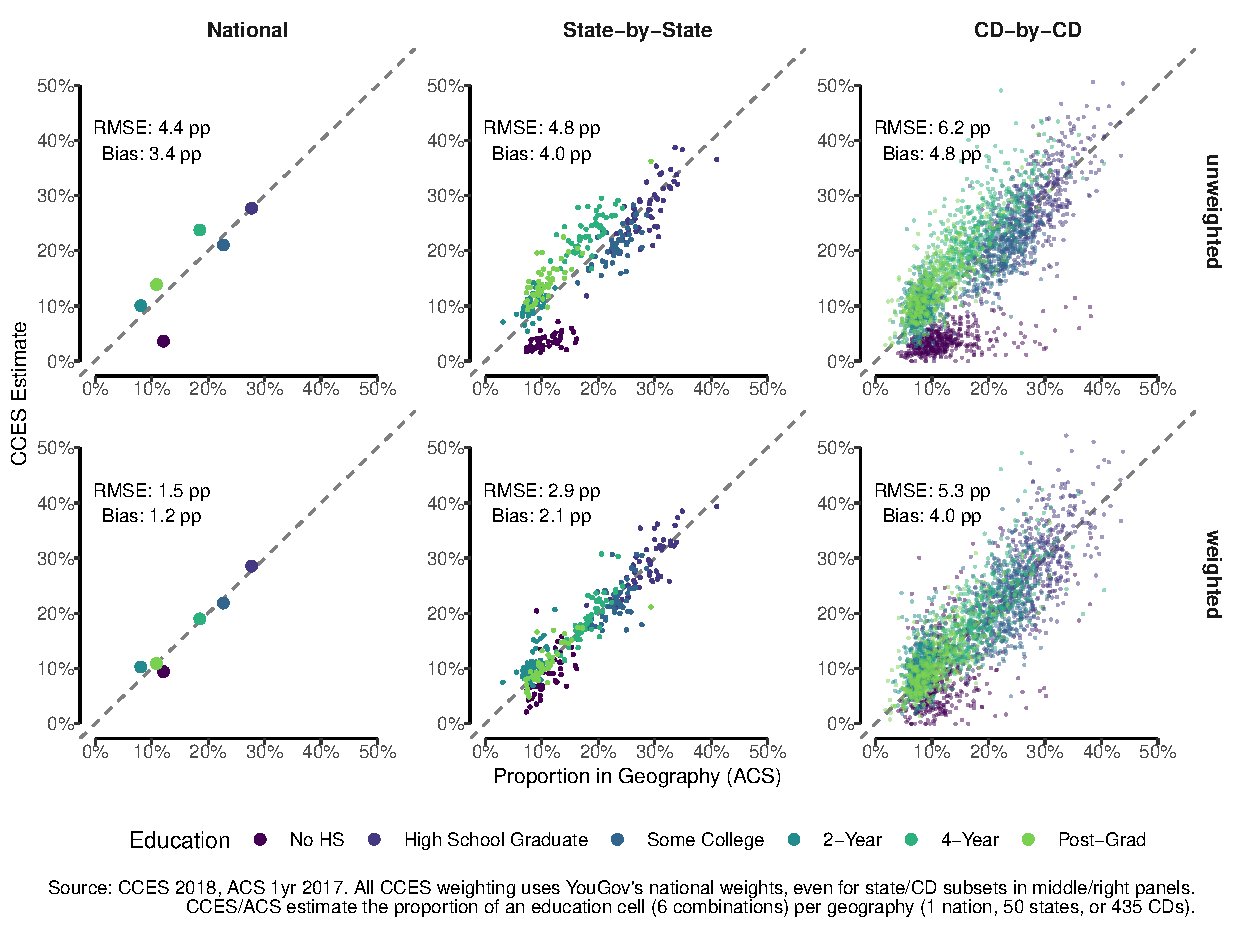
\includegraphics[width = 0.9\textwidth]{figures/educfrac-comparisons.pdf}
\end{figure}

\FloatBarrier

We next take a look not only at education, but the representativeness in terms of education-gender-age joint distributions. YouGov weights on first moments and (presumably two-way) interactions, so their weighted are not guaranteed to hold for three-way joint distributions.  Figure \ref{fig:cellfrac-ed-age-sex} shows those quantities of interest, proliferating the number of points to examine. We find:

\smallskip 
\begin{enumerate}
\item National estimates improve about as much as in Figure \ref{fig:cellfrac-ed} in ratio terms.
\item State estimates also improve somewhat, but not by much (8 percent reduction in RMSE, as opposed to 40 percent in the marginal distribution case).
\item District estimates do not improve, and its bias \emph{increases} slightly by 0.08 percentage points. The bias variance decomposition suggests that the variance has increased as well.
\item Some of the outliers in the state estimate suggests that the YouGov national weights up-weight some state-demographic cells in a way that makes them less representative of the state. 
\end{enumerate}

\begin{figure}[bt!h]
\centering
\caption{Representativeness of samples at different levels of geographies, education \(\times\) age \(\times\) gender fraction \label{fig:cellfrac-ed-age-sex}}
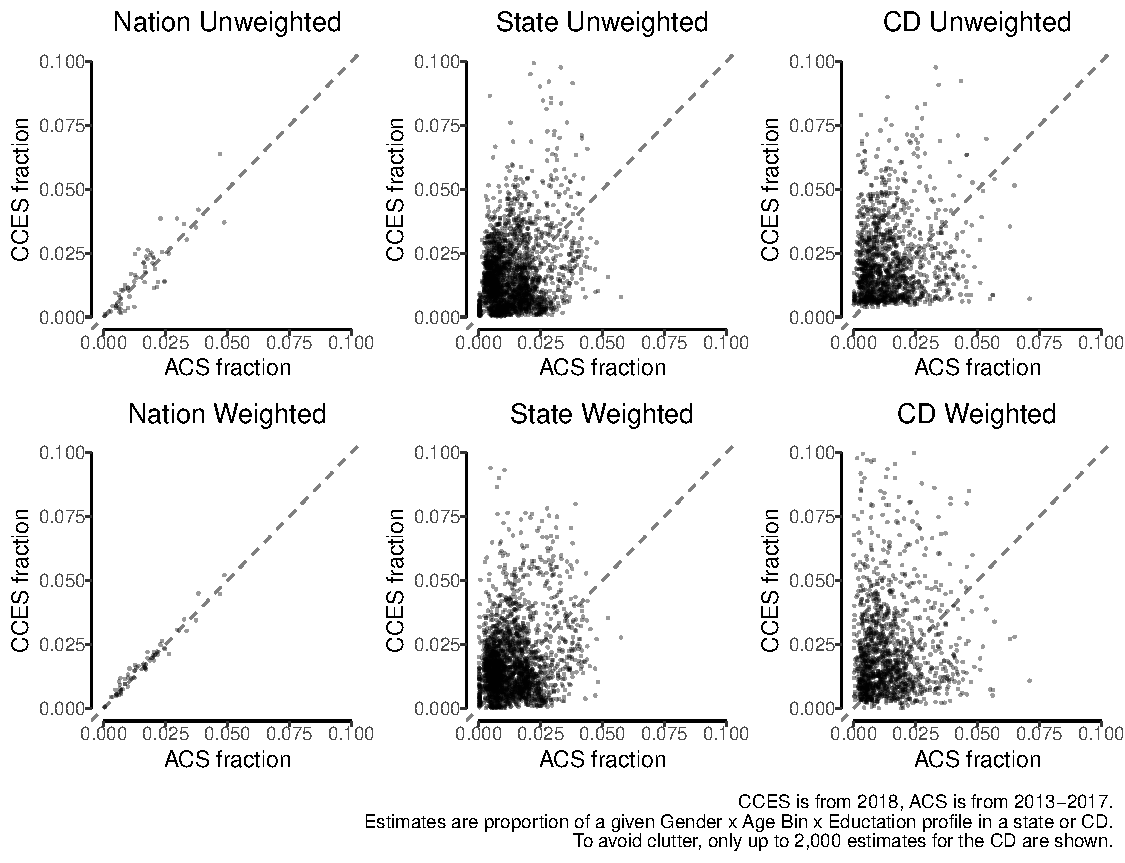
\includegraphics[width = \textwidth]{figures/cellfrac-comparisons.png}
\end{figure}

\FloatBarrier
\newpage

\section{State Weights Results \label{sec:res-state}}

Do weights that are specifically targeted to match on the state-specific moments improve representativeness? How does it improve representativeness at levels larger lower than its target? Figure \ref{fig:rim-comparisons} shows figures analogous to the prior figures.

\medskip

\begin{enumerate}
\item As expected, the weights coerce the margins to match the population targets.
\item Although each state subsample's weights is computed separately, its concatenation makes national estimates representatives too. 
\item At the smaller district level, the marginal estimates have also improved, and slightly outperform the YouGov weights.
\item However, rim weights do not necessarily improve representativeness of joint distributions. The bottom panel shows that those estimates are about as representative as those with YouGov weights, perhaps by reducing the variance.
\end{enumerate}
\begin{figure}[bt!h]
\centering
\caption{Representativeness with custom state-by-state rim weights \label{fig:rim-comparisons}}
\includegraphics[width = 0.9\textwidth]{figures/educfrac-rim-comparisons.pdf}
\includegraphics[width = 0.9\textwidth]{figures/cellfrac-rim-comparisons.png}
\end{figure}

\end{document}



 